%%% Chapter 5 - Hardware Implementation %%%

\chapter{Hardware implementation} \label{ch:hardware_implementation}
To this date, sustainable energy sources have become an area of worldwide focus in an attempt to reduce the environmental impact due to emissions of $CO_{2}$ and other greenhouse gasses. The development of competitive systems to exploit renewable energy sources is the best alternative to reduce the use of fossil fuels for the production of electricity. Over the last years there has been a considerable increase in electricity production from renewable energy sources being the fastest growing sectors wind and solar energy. In 2017, photovoltaic generation was the renewable energy source which experienced the highest increase in newly installed capacity. The total installed capacity reached approximately 402 GW\cite{global}. %[http://www.ren21.net/wp-content/uploads/2018/06/17-8652_GSR2018_FullReport_web_-1.pdf] 

Photovoltaic (PV) is referred to the production of electricity in the form of direct current (DC) directly from sunlight shining on solar cells. Solar cells are semiconductor devices which typically can produce around 0.5 V DC so they are series connected to form a PV panel which can also be connected to other PV panels resulting in a PV array \cite{handbook}. This way, according to the system's requirements, the PV panels can be interconnected in series or parallel in order to get at the output a higher voltage or current, respectively. Connecting PV panels either in series or parallel will result in an increase of the system's overall electricity production. %[http://www.sabz-energy.com/solar%20electricity%20handbook%202017.pdf] 

Nevertheless, it is essential to keep into consideration the mismatches that may appear on the power generated by the different PV panels. This will result in losses in the PV system and thus in a lower efficiency. Mismatches may lead to uneven power generation. These can be caused to partial shading, manufacturing tolerances, defects in the PV modules due to weather conditions and ageing among others. Even a small mismatch in one of the PV modules can result in a very high reduction of the power production from the entire PV array \cite{MPPmismatch}. Mismatch losses in a PV system can be reduced by forcing every PV module to work at its MPP by using a technique known as Maximum Power Point Tracking (MPPT). This can be reached by using electronic devices called Module Integrated Converters (MICs). MICs consist on DC-AC micro inverters or DC-DC converters that incorporate a MPPT controller unit to ensure that the output power of the MIC is the one corresponding to the MPP of the PV module.%[https://www.researchgate.net/publication/43248773_Study_on_MPP_mismatch_losses_in_photovoltaic_applications] 

\section{Selection of commercial components}

\subsection{Passive components}
\todo{WE MADE A MISTAKE HERE, NEED TO EXPLAIN WHY WE OBTAINED A MUCH LOWER VALUE. MAYBE TO EMULATE THE CAPACITANCE AT THE INVERTER.}
For the output capacitor a $820\mu F$\todo{in equation 4.9 we have a completely different value.. why? Stef } has been used \cite{cout}. An electrolytic capacitor has mostly been chosen because of small size and low cost. The voltage rating is 250V which is a fine margin to the 90V that is the highest possible output. \todo{with max 90V a much lower voltage rating could have been chosen! margin is again not the reason for this value, true that maybe we did oversize it when designing. AT} \todo{well not saying that the margin is the reason. Just mentioning it. Can't see that is a problem? JK}
Achieving the necessary input capacitance with only one capacitor would result in very big size of the component, therefore four electrolytic capacitors of $470\mu F$ \cite{cin} are placed in parallel to get a summed capacitance of $1.880\mu F$ \todo{1.8 mF isn't it? Stef}. The rating for these is 100V which has been chosen in case the output is connected to the input by accident. In this case that will not ruin the input capacitor. These ESR resistances\todo{which ESR resistance? and how do you get this value?Stef} will be about $0.047\Omega$. Both input and output capacitor have a capacitance higher than the calculated worst case. This is because the converter maybe in the future will have a buck-boost mode as well. And in this mode the capacitance can get a bit higher. \todo{I think this is not the best way to introduce the buck boost possibil<ity. AT}
Both for the input and output a $100nF$ and a $1\mu F$ \todo{where do these values come from?Stef} capacitors are placed in parallel. This is mostly done because the big electrolytic capacitors is not able to supply the needed current at higher frequencies. With these extra capacitors the high frequency transients should be filtered away.

The inductor for first iteration \todo{What does first iteration mean? have we explained it previously? AT} will be with an inductance of around 1mH, \todo{exact value should be determined JK} because that is an inductor the supervisors had in-house already.

\subsection{Swithing circuitry}
\subsection{Switching circuitry}

Selecting the switching circuitry consists of four different parts, switches, heat sink, drivers, and optocouplers. Additional support circuitry will be designed, when selecting the commercial components.

\subsubsection{Switch sizing} \label{switch_sizing}
The system must regulate the power flow in order to maximize the power generation. In order to achieve this, the system includes switches that control the current flow. The switches consist of MOSFET devices. The switching frequency of the system is selected to be $50kHz$. Although the market has IGBT which can switch at $50kHz$, MOSFET devices allow lower losses than IGBTs for system's current rating \cite{mosfet_igbt_switching_loss} \cite{igbt_or_mosfet}.


The maximum output voltage of the system is $90V$, however the voltage rating of the transistors was set to $150V$ in order to consider a safety margin, and thus, increase the reliability. The peak current through the transistors happens when the buck mode is active and the maximum number of MICs are connected in series. The peak current is equal to $14A$. In order to reduce the conduction losses and the heat sink size, a low on resistance is desired shown in equation \ref{conduction_losses_eq}\cite{mosfet_losses}. These constraints were used when searching for the commercial component. The chosen device is the IPB200N15N3. It exhibits the features seen in table \ref{mosfet_features}.


\begin{table}[htbp]
	\centering
	\begin{tabular}{|p{6cm}|>{\centering}p{6cm}|}
		\hline
		\rowcolor{lightgray}\multicolumn{2}{|l|}{ \textbf{Maximum ratings}} \\ \hline
		Continuous $I_{D}$ & 40 [A]  \tabularnewline \hline
		$V_{GS}$ & $\pm$ 20 [V]  \tabularnewline \hline
		Power dissipation & 150 [W]  \tabularnewline \hline
		$V_{DS}$ & 150 [V]  \tabularnewline \hline
		$R_{DS} $ & 20 [m$\Omega$]  \tabularnewline \hline
		\rowcolor{lightgray}\multicolumn{2}{|l|}{ \textbf{Other values of interest}} \\ \hline
		$C_{iss}$ & 1820 [pF]  \tabularnewline \hline
		Package & D2PAK  \tabularnewline \hline
		$V_{th} $ $(V_{GS} = 3 V)$ & 3 [V]  \tabularnewline \hline
		$V_{th} $ $(V_{GS} = 36 V)$ & 4.7 [V]  \tabularnewline \hline
		$R_{Gate} $ & 2.4 [$\Omega$] 
		\tabularnewline \hline
		$R_{th ja} $ & 75 [$\dec C /W$]  \tabularnewline \hline
	
	\end{tabular}
	\caption{MOSFET figures of merit. T = 25 $\decC$ \cite{mosfet_datasheet}.}
	\label{mosfet_features}
\end{table}

\subsubsection{Heat sink sizing}

The procedure followed for validating the heat sink might be seen at figure \ref{heat_sink_validation_procedure}. If the total temperature increase is within switch's safe operating area, then the heat sink is providing enough heat dissipation.

\begin{figure}[htbp]
	\begin{center}
		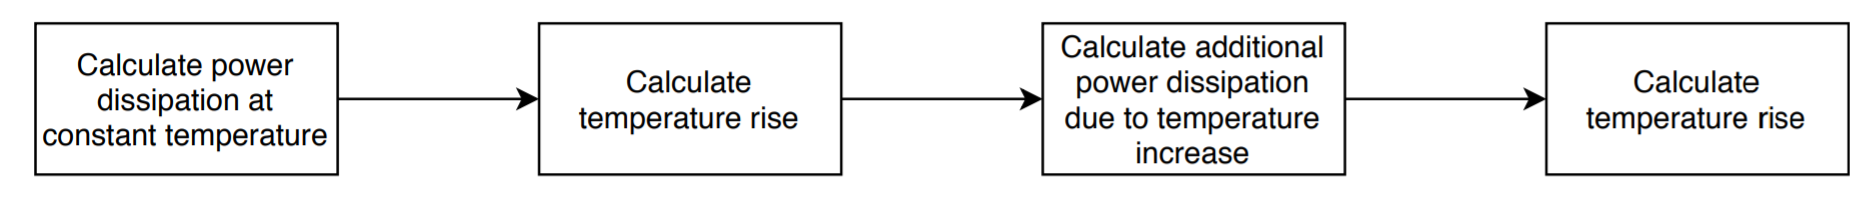
\includegraphics[width=\textwidth]{../Pictures/P1/Component_sizing/heat_sink_validation_procedure.png}
		\caption{Heat sink validation procedure.}
		\label{heat_sink_validation_procedure}
	\end{center}	
\end{figure}

The power dissipated in the switches is equal to the sum of the conduction losses and the switching losses. The conduction losses might be calculated  as seen in equation \ref{conduction_losses_eq}.

\begin{equation} \label{conduction_losses_eq}
P_{cond} = i(t)^2 \cdot R_{DS}
\end{equation}

The switching losses depend upon the switching frequency and the transistor's manufacturing characteristics \cite{mosfet_losses}. In order to calculate the value, the MOSFET's SPICE model is available in the LTspice default library. The next step was to perform the simulation of the system. The system was simulated in both buck and boost modes. Special attention was put into the dead-band between PWM signals of different switches, to avoid current shoot through. After simulating, the average power dissipation under steady state was calculated in both modes. Within every mode, the simulation was performed under the most unfavorable conditions, this is: buck's output is 24 V and boost's output is 90 V. The results can be seen in table \ref{mosfet_final_dissipation}, column 1.

The datasheet shows that the $R_{DS}$ variation is mainly dependent on the temperature\cite{mosfet_datasheet}. The models found neglect the temperature difference. 
Then, in order to get an approximated value considering temperature, the procedure will be to calculate the total losses at constant temperature using the SPICE model. 
Then add the additional conduction losses due to the increase of the resistance, as expressed by equation \ref{total_losses}.

\begin{equation} \label{total_losses}
\overline{P} = \overline{P_{loss, T = K}} + \overline{i(t)^2 \cdot \Updelta R_{DS}}
\end{equation}

Now the junction temperature based on the power dissipation, calculated using the SPICE model, is calculated. The ambient temperature is set to 50 $\decC$, which is considered a realistic scenario. The thermal circuit can be seen in figure \ref{thermal_circuit}. The next step is to choose a commercial heat sink. The constraints are thermal resistance, size and price. TDEX6015/TH was found. Its features might be found in table \ref{heatsink_features}. The switches temperature will be analysed in order to validate the heat sink. The analysis considers all the transistors as a single power source.

\begin{figure}[H]
	\begin{center}
		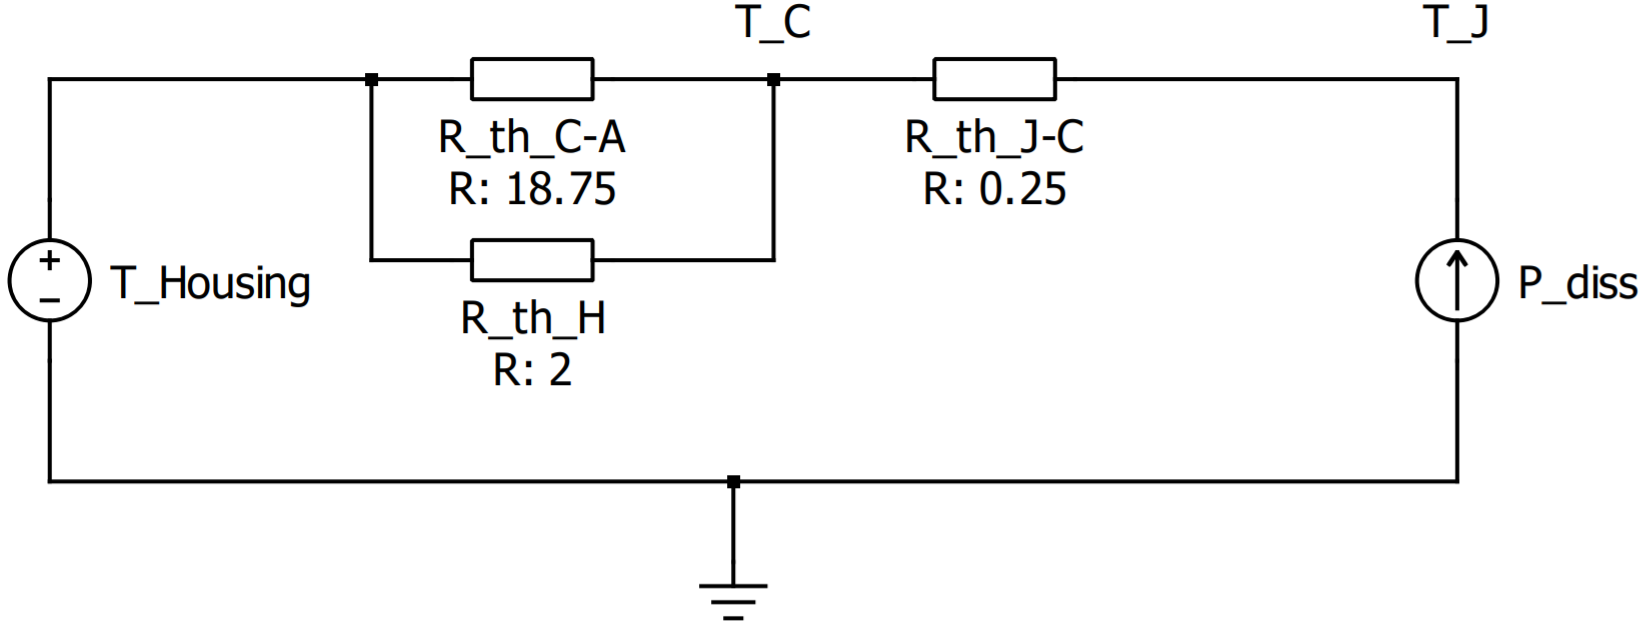
\includegraphics[width=0.7\textwidth]{../Pictures/thermal_circuit.png}
		\caption{Thermal circuit used for sizing the heat sink}
		\label{thermal_circuit}
	\end{center}	
\end{figure}

\begin{equation} \label{switch_temperature}
T_{J} = T_{housing} + \overline{P_{loss, T = k}} \cdot  R_{thermal}
\end{equation}


If no heat sink were used, according to equation \ref{switch_temperature}, the junction temperature would become too high and the components would be damaged (see equation \ref{temperature_without_heatsink}). This is mainly explained due to the fact that the thermal resistance between junction and ambient of the transistor is as high as 75 $\decC / W$, information about the power dissipation can be found in table \ref{mosfet_final_dissipation}.

\begin{equation} \label{temperature_without_heatsink}
T_{J} = 50 \decC + 5.54 W \cdot 75 \frac{\decC}{W} = 465.5 \decC
\end{equation}


\begin{table}[htbp]
	\centering
	\begin{tabular}{|p{4cm}|>{\centering}p{8cm}|}
		\hline
		\rowcolor{lightgray}\multicolumn{2}{|l|}{ \textbf{Features}} \\ \hline
		Size & 60x60x16 [mm]  \tabularnewline \hline
		Thermal resistance & 2.06 [$\dec C/W$]  \tabularnewline \hline
		
	\end{tabular}
	\caption{Heat sink figures of merit \cite{heatsink_datasheet}.}
	\label{heatsink_features}
\end{table}


\begin{equation} \label{switch_temperature_w_values}
T_{J} = 50 \decC + 5.54 W \cdot  2.06\frac{\decC}{W} = 61.41 \decC
\end{equation}

The drain-to-source resistance increase is calculated as explained in equation \ref{delta_resistance}. The resistance difference is relatively small. The resistor at every temperature was collected from the component data sheet.

\begin{equation} \label{delta_resistance}
\Updelta R_{DS} = |R_{DS, T = 20 \decC} - R_{DS, T = 61.41\decC}| = 4\; m \Omega
\end{equation}

\begin{table}[]
	\centering
	\begin{tabular}{|l|l|l|l|}
		\hline
		\rowcolor[HTML]{C0C0C0} 
		\multicolumn{4}{|c|}{\cellcolor[HTML]{C0C0C0}\textbf{Switches power dissipation}}                                                   \\ \hline
		\rowcolor[HTML]{C0C0C0} 
		Switch         & $\overline{P_{loss, T = K}}$ {[}W{]} & $ \overline{i(t)^2 \cdot \Updelta R_{DS}}$ {[}W{]} & \textbf{Total {[}W{]}} \\ \hline
		\multicolumn{4}{|l|}{Buck mode}                                                                                                     \\ \hline
		M1             & 2.91                                 & 0.39                                               & \textbf{3.30}          \\ \hline
		M2             & 0.82                                 & 0.21                                               & \textbf{1.03}          \\ \hline
		M3             & 1.81                                 & 0.58                                               & \textbf{2.39}          \\ \hline
		M4             & 0                                    & 0                                                  & \textbf{0}             \\ \hline
		\textbf{Total} & 5.54                                 & 1.18                                               & \textbf{6.72}          \\ \hline
		\multicolumn{4}{|l|}{Boost mode}                                                                                                    \\ \hline
		M1             & 0.69                                 & 0.28                                               & \textbf{0.97}          \\ \hline
		M2             & 0                                    & 0                                                  & \textbf{0}             \\ \hline
		M3             & 0.48                                 & 0.12                                               & \textbf{0.6}           \\ \hline
		M4             & 3.31                                 & 0.18                                               & \textbf{3.49}          \\ \hline
		\textbf{Total} & 4.48                                 & 0.58                                               & \textbf{5.06}          \\ \hline
	\end{tabular}
\caption{Power dissipation analysis. Column 1, average power dissipation at constant 25 $\decC$ temperature. Column 2, extra power dissipation due to the increase of temperature.}
\label{mosfet_final_dissipation}
\end{table}


The full power dissipation values can be found on table \ref{mosfet_final_dissipation}. To achieve an exact result, an iterative process should be followed. However, after the first iteration, the change ratio is extremely small and then, neglected. Now that the power dissipation has been calculated, the junction temperature must be checked in order to confirm that the heat sink has been properly sized. Equation \ref{switch_temperature} is used, substitution of values leads to equation \ref{switch_temperature_w_values_2}. The difference is fairly small and the junction temperature remains within safe area. Then, TDEX6015/TH has been validated as a proper heat sink.

\begin{equation} \label{switch_temperature_w_values_2}
T_{J} = 50 \decC + 6.72 W \cdot  2.06 \frac{\decC}{W} = 63.84 \decC
\end{equation}
\subsubsection{Drivers and optocouplers}  \label{driver}

The control signal is generated by the control platform, which consists on a Plexim RTbox. In order to provide galvanic isolation between the converter and the control signal generator, optocouplers are used. The chosen optocoupler is the ACPL-P302. This optocoupler includes output signal circuitry which allows saving a pull-up or pull-down resistor. The IC is not an open collector device. Its main features might be seen at \ref{opto_features}.

\begin{table}[H]
	\centering
	\begin{tabular}{|p{6cm}|>{\centering}p{8cm}|}
		\hline
		\rowcolor{lightgray}\multicolumn{2}{|l|}{ \textbf{Maximum ratings}} \\ \hline
		Supply voltage & 35 [V]  \tabularnewline \hline
		Average input current & 25 [mA]  \tabularnewline \hline
		Peak output current & 0.4 [A]  \tabularnewline \hline
		\rowcolor{lightgray}\multicolumn{2}{|l|}{ \textbf{Other values of interest}} \\ \hline
		Input forward voltage & 1.5 [V]  \tabularnewline \hline
		Package & SSOIC6  \tabularnewline \hline
	\end{tabular}
	\caption{Optocoupler figures of merit.
	\cite{opto_datasheet}}
	\label{opto_features}
\end{table}

The signal from the optocoupler has to be amplified in order to drive the switches. The driver provides voltage amplification and current capability. The chosen IC to perform the task is NCP81074B. Find in table \ref{driver_features} its main features. 

\begin{table}[htbp]
	\centering
	\begin{tabular}{|p{6cm}|>{\centering}p{8cm}|}
		\hline
		\rowcolor{lightgray}\multicolumn{2}{|l|}{ \textbf{Maximum ratings}} \\ \hline
		Supply voltage & 24 [V]  \tabularnewline \hline
		Output current (pulse < 0.5 $\mu$s) & 10 [A]  \tabularnewline \hline		
		Reverse current (pulse < 1 $\mu$s) & 10 [A]  \tabularnewline \hline
		Input signal voltage & -6 to 24 [V]  \tabularnewline \hline
		\rowcolor{lightgray}\multicolumn{2}{|l|}{ \textbf{Other values of interest}} \\ \hline
		Output resistance & 0.4 [$\Omega$]  \tabularnewline \hline
		Package & SOIC8  \tabularnewline \hline
	\end{tabular}
	\caption{Driver figures of merit.
		\cite{driver_datasheet}}
	\label{driver_features}
\end{table}

The MOSFET is a voltage controlled device, the relationship between $V_{GS}$ and $V_{th}$ sets the drain to source maximum current, as seen in figure \ref{ids_vgs}.

\begin{figure}[htbp]
	\begin{center}
		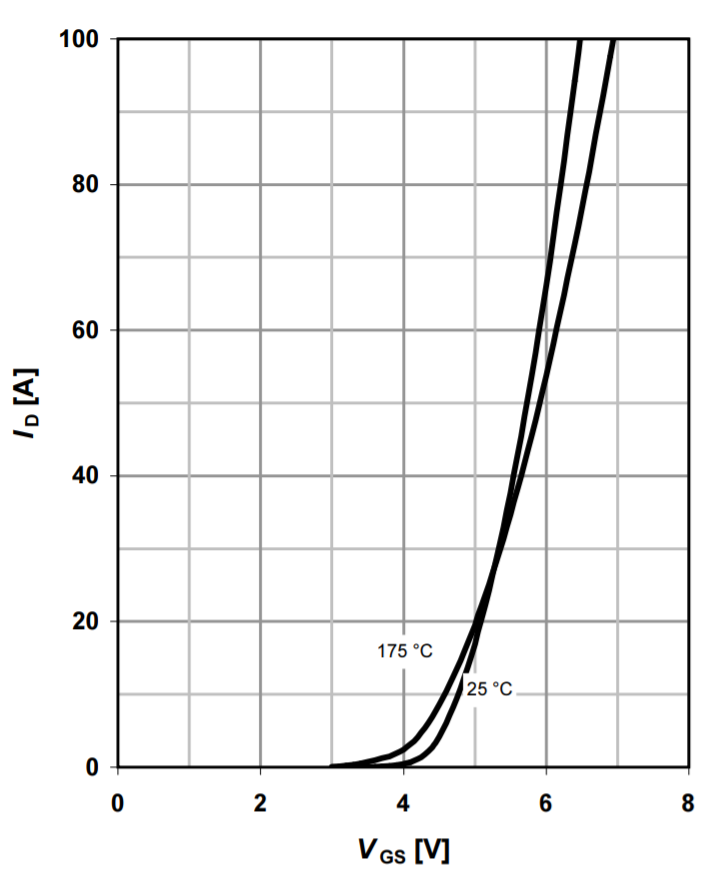
\includegraphics[width=0.4\textwidth]{../Pictures/P1/Component_sizing/ids_against_vgs.png}
		\caption{Drain to source current against gate to source voltage $(V_{DS} > 2 \cdot I_{D}\cdot R_{DSon}) $.}
		\label{ids_vgs}
	\end{center}
\end{figure}

The dynamics of the switching can be modelled as a RC circuit, see figure \ref{mosfet_rc_gate}. Both $R_{driver \; out}$ and $R_{MOSFET}$ are directly obtained from the components' data sheets, $C_{iss}$ is also available in the MOSFET data sheet as input capacitance.



\begin{figure}[H]
	\begin{center}
		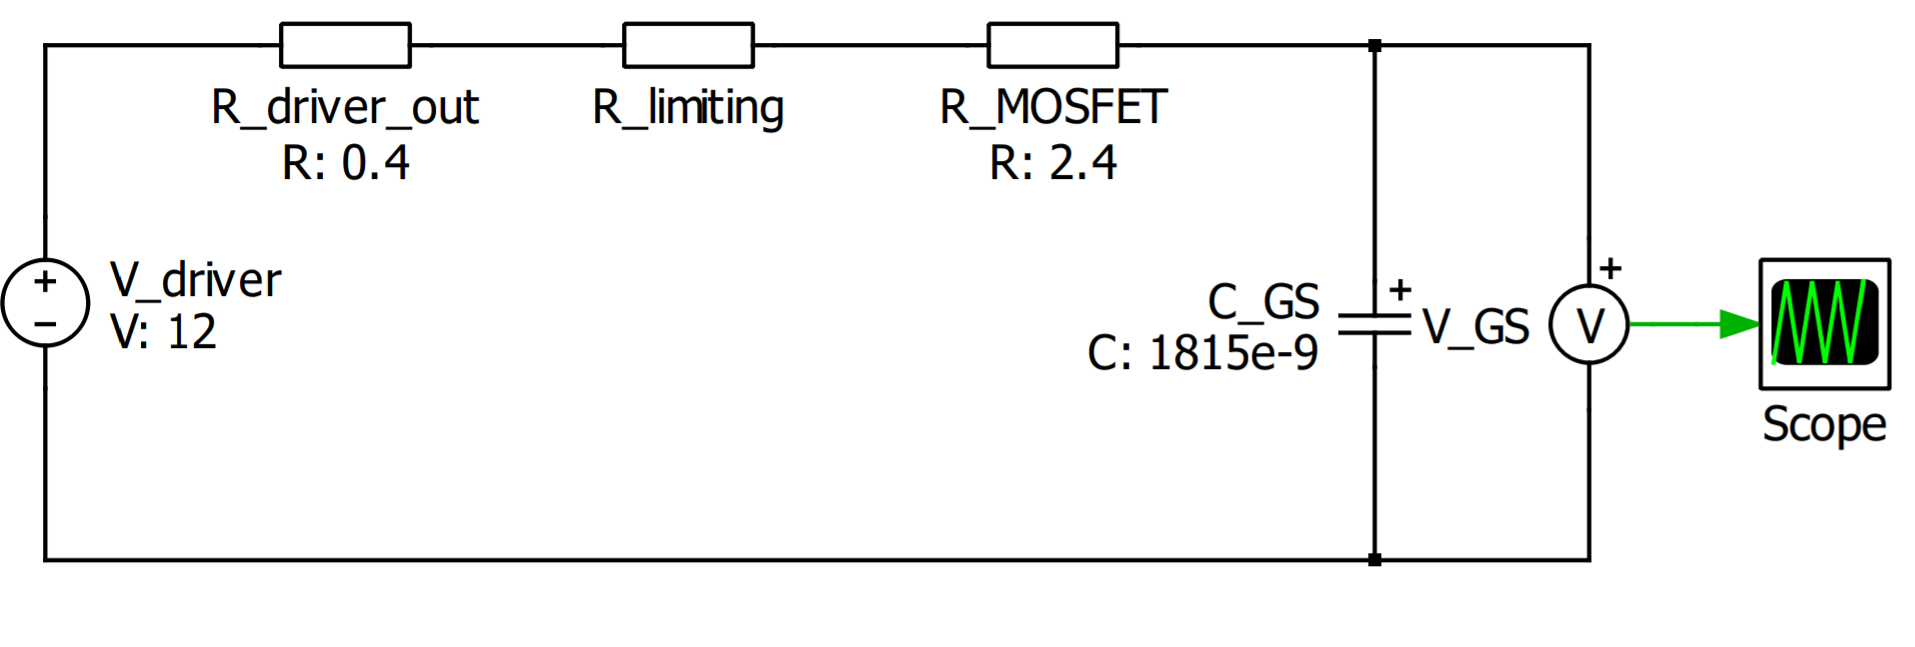
\includegraphics[width=0.8\textwidth]{../Pictures/P1/Component_sizing/driver_resistor_sizing.png}
		\caption{Simplified circuit used to model the MOSFET switching dynamics.}
		\label{mosfet_rc_gate}
	\end{center}	
\end{figure}

The time where the gate capacitor voltage reaches the threshold voltage produces a propagation delay from the driver output to the actual beginning of the MOSFET switching. In order to size the limiting resistor of the RC circuit, a time constraint was needed. This time constraint was arbitrarily set in relation with the switching frequency as described in equation \ref{time_constraint}. The 0.1\% constraint results in a limiting resistor of 20 $\Omega$. The average power dissipation, according to simulation, is 13 mW. This value is well under the power rating of the used SMD resistor with 1206 package, which is 250 mW. However the peak power dissipation was also considered, as it is relatively high. According to simulation, the peak is equal to 5.4 W, see figure \ref{gate_resistor_power_dissipation}. Although this value exceeds the resistor power rating, some manufacturers agree that the peak power dissipation in pulses shorter than 10 $\mu$s using 1206 resistors is 19 W \cite{pulse_withstanding_chip_resistors}, \cite{gate_driver_design_infineon}. Then the peak power dissipated shouldn't harm the component. Once the prototype is built, the thermal behaviour of the component is analysed with a thermal camera. \todo{did we get to do this?}

\begin{equation} \label{time_constraint}
t_{delay} = t\big\rvert_{V_{GS} = V_{th}} =\frac{T_{sw}}{1000} = 0.1 \% \;\; of \;\; T_{sw} = 20 \; ns
\end{equation}


\begin{figure}[H]
	\begin{center}
		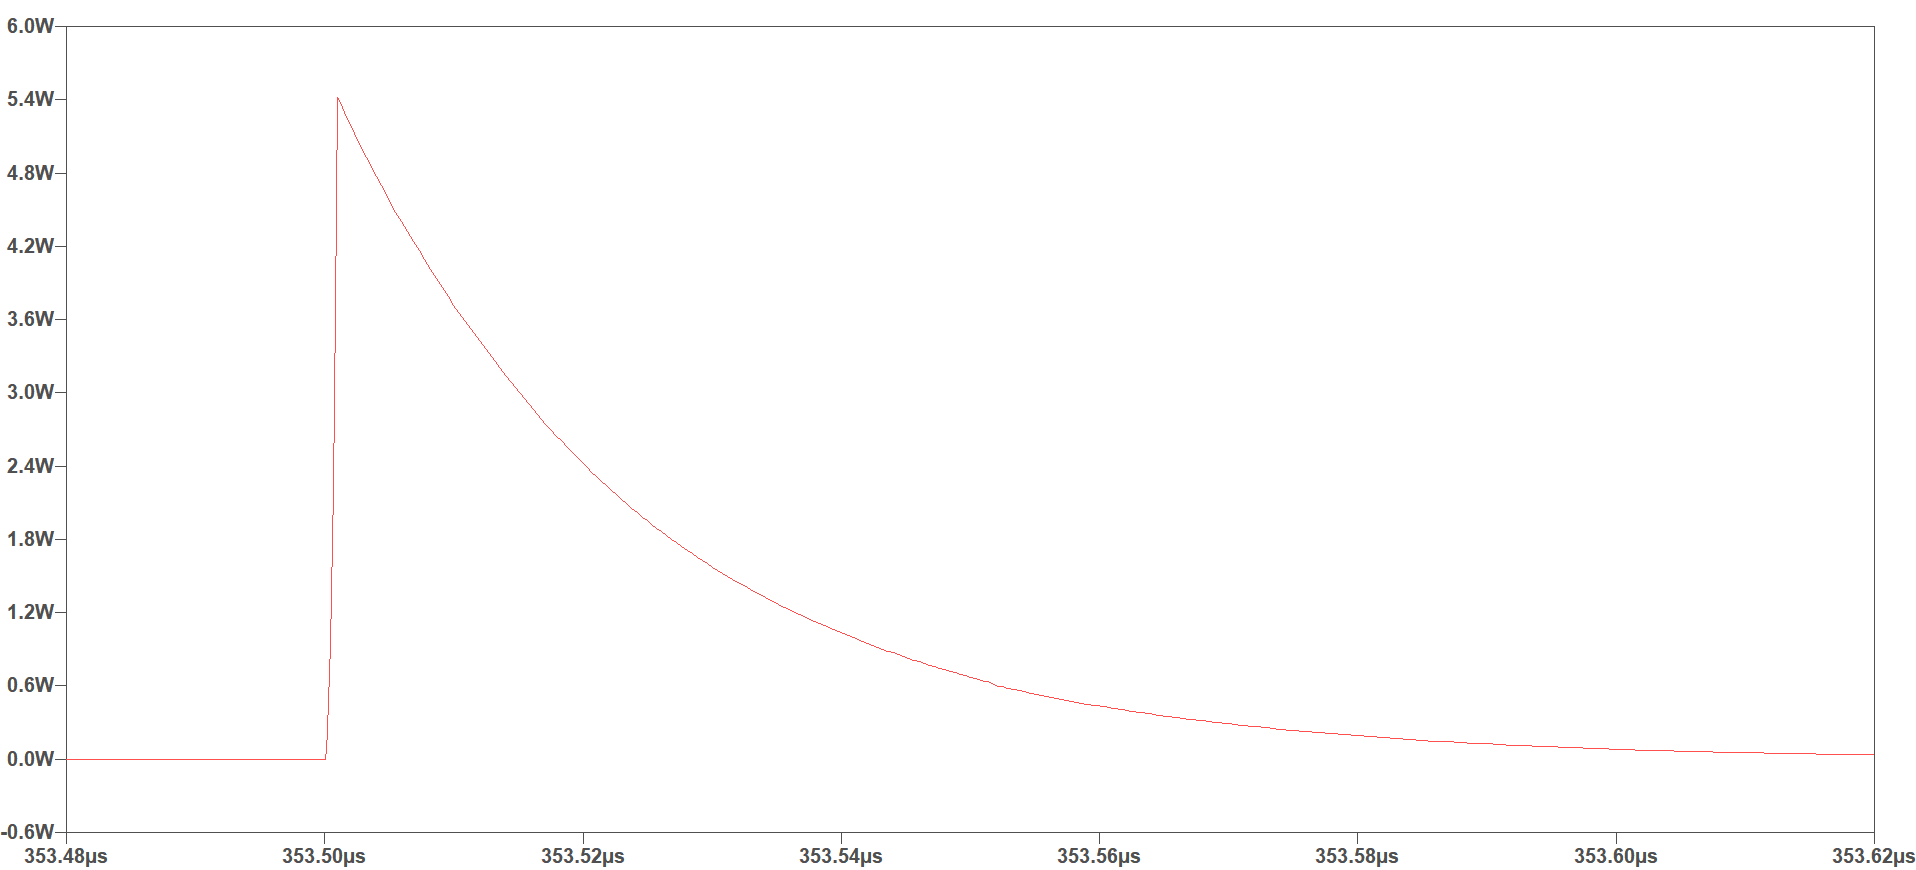
\includegraphics[width=1.15\textwidth]{../Pictures/P1/Component_sizing/Gate_resistor_power_dissipation.png}
		\caption{Detail of the power dissipated at R\_limiting during MOSFET turn-on.}
		\label{gate_resistor_power_dissipation}
	\end{center}	
\end{figure}
 
The implemented topology has the peculiarity that two MOSFETs' sources are not directly connected to ground. As explained previously, it is the Gate to Source voltage that determines whether the transistor is conducting or not. In order to get a floating voltage in the high side drivers, one option is to have isolated supplies for those drivers. The ground of this isolated supplies will be tied to the low side MOSFET's drain. More explanation regarding the isolated supplies might be found at \ref{power_supplies}.

In case that the drivers were damaged, the residual voltage of the transistor's gate might become undefined, then, in order to ensure that the switch is off, a pull down resistor is added between the gate and the source of the transistor. This resistor has been sized to 1 M$\Omega$, which discharges the gate voltage from 12 V to below its threshold in less than 3 ms.


%% These sections describes the design and implementation of the chosen sensors.

\subsection{Sensing circuitry} \label{sensors}
To implement the MPPT it is necessary to measure the output voltage and current of the PV module. These measurements will be obtained by placing a voltage and current sensor. A second voltage sensor will be implemented to measure the output voltage of the DC-DC coverter, for possible future use. 

To protect the RT Box, it has been chosen to fully isolate it from the power stage of the converter. To do so, the sensors will have to include isolation between input and output.  

%%% Voltage sensors %%%
\subsection{Input voltage sensor} \label{voltage_sensors}
The voltage sensor selected is ACPL-C870 \cite{voltage_sensor}. This sensor includes optical isolation amplifiers, which makes it well suited for isolated voltage sensing. The amplifier includes unity gain $1V/V$ amplification, with an accuracy at $\pm 3 \%$. Figure \ref{fig:voltage_sensors_placement} shows the placement of the two voltage sensors, where $V_{in}$ and $V_{out}$ are the input and output sensor respectively. 

\begin{figure}[htbp]
	\begin{center}
		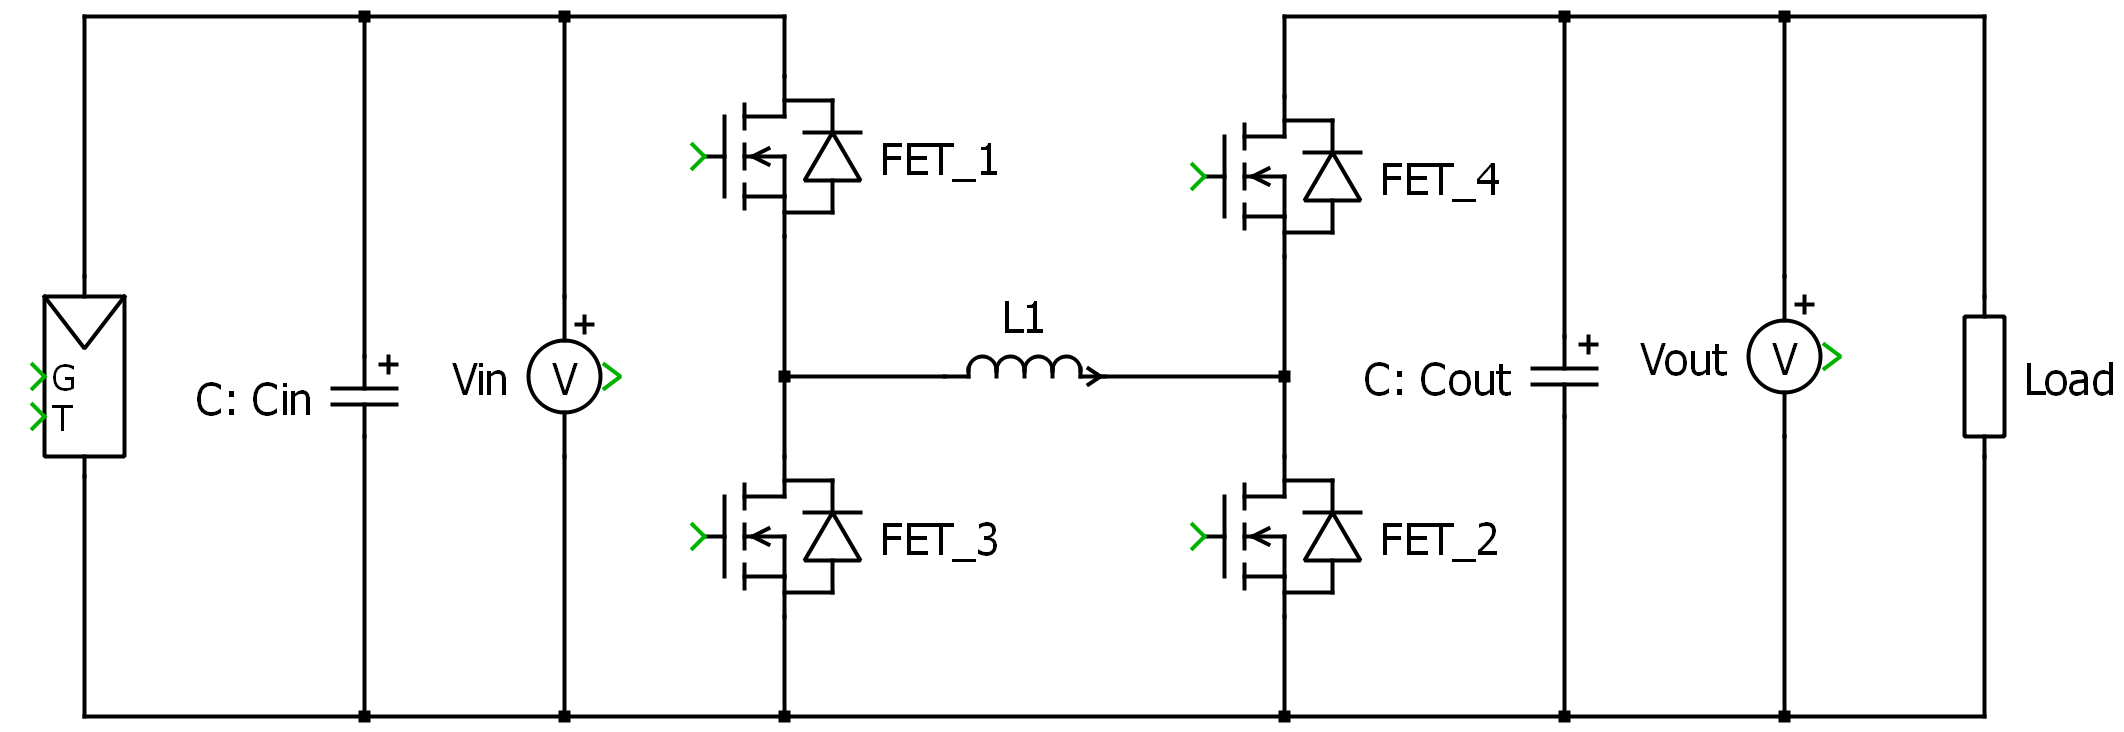
\includegraphics[width=0.7\linewidth]{../Pictures/P1/Sensors/voltage_sensors_placement.PNG}
		\caption{Voltage sensors placement}
		\label{fig:voltage_sensors_placement}
	\end{center}
\end{figure} 

\subsubsection{Voltage divider}
The input voltage at the voltage sensor is recommended to be in the range of $0V-2V$. To divide the measured voltage into that range, a voltage divider will be implemented. 

The maximum output voltage of the PV-module is the open-circuit voltage at $45.2V$. To achieve a safety margin and to make the converter adaptable to other types of PV-modules, $50V$ has been selected. The current flow in the voltage divider has been set at $1mA$, to secure a insignificant power loss. The resistors can be calculated with the following equations:
\begin{equation} \label{voltage_divider_R17_in}
	R_{17} = \frac{V_{in,max}-V_{out}}{I} = \frac{50V-2V}{1mA} = 48k\Omega
\end{equation}

\begin{equation} \label{voltage_divider_R18_in}
	V_{out} = V_{in,max} \cdot \frac{R_{18}}{R_{17}+R_{18}} \Rightarrow 2V = 50V \cdot \frac{R_{18}}{48k\Omega+R_{18}}
\end{equation}
\begin{center}
	$R_{18} = 1.958k\Omega$
\end{center}

To achieve these resistor values $R_{17} = 47k\Omega$ and $R_{18} = 2k\Omega$ have been chosen. 

\subsubsection{Filtering} \label{voltage_sensor_filter}
For a stable MPPT control, the measured voltage must have a very low ripple. To ensure this, a low-pass RC filter with a corner frequency at $500Hz$, will be placed between the voltage divider and the sensor. The resistor of the filter will be $R_1$ in the voltage divider. The capacitor will calculated as followed in equation \ref{voltage_sensor_in_filter_cap}:
\begin{equation} \label{voltage_sensor_in_filter_cap}
	C_{17} = \frac{1}{2\pi \cdot f_c \cdot R_{17}} = \frac{1}{2 \pi \cdot 500Hz \cdot 47k\Omega} = 6.7nF
\end{equation}

To achieve the capacitance $C_{17} = 6.6nF$ has been chosen. 

\subsubsection{Amplification} \label{voltage_sensor_amplification}
The input range of the ADC in the RT-Box is $0V-5V$. To take advantage of the entire range an amplifier will be implemented. The output of the voltage sensor is differential with an offset at $1.23V$. Therefore a differential amplifier will be implemented using a LMC6484 quad operational amplifier \cite{sensor_opamp}. By using a quad amplifier, the same IC can be used for the output voltage sensor and the current sensor.

The resistors of the differential amplifier will be sized with equation \ref{voltage_sensor_gain}.
\begin{equation} \label{voltage_sensor_gain}
	V_{out} = \frac{R_{22}}{R_{20}} \cdot (V_2-V_1)
\end{equation}

Where $V_2-V_1$ is the difference between the output pins of the voltage sensor. With unity gain in the voltage sensor, the maximum difference at the output will be $2V$. This should correspond to the maximum input voltage of the ADC at $5V$. $R_1$ is selected to be $11k\Omega$. The resistor $R_{22}$ is now calculated using equation \ref{voltage_sensor_gain}.
\begin{equation}
	5V = \frac{R_{22}}{11k\Omega} \cdot 2V
\end{equation}
\begin{center}
	$R_{22} = 27.5k\Omega$
\end{center}
To achieve the value of $R_{22}$ it's rounded to be $27k\Omega$. Furthermore $R_{19} = R_{20}$ and $R_{21} = R_{22}$, to get a balanced differential amplifier.

\subsubsection{The circuit}
The circuit regarding the input voltage measurement is shown at figure \ref{fig:input_voltage_sensor_circuit}. $V_{in}$ is the measured voltage from the PV-module. The points $OA1_+$ and $OA1_-$ are connected to the non-inverting and inverting input of the amplifier respectively. $OA1_{out}$ is connected to the output of the amplifier. $C_{15}$ and $C_{16}$ are decoupling capacitors for the two supply voltages. 

\begin{figure}[H]
	\begin{center}
		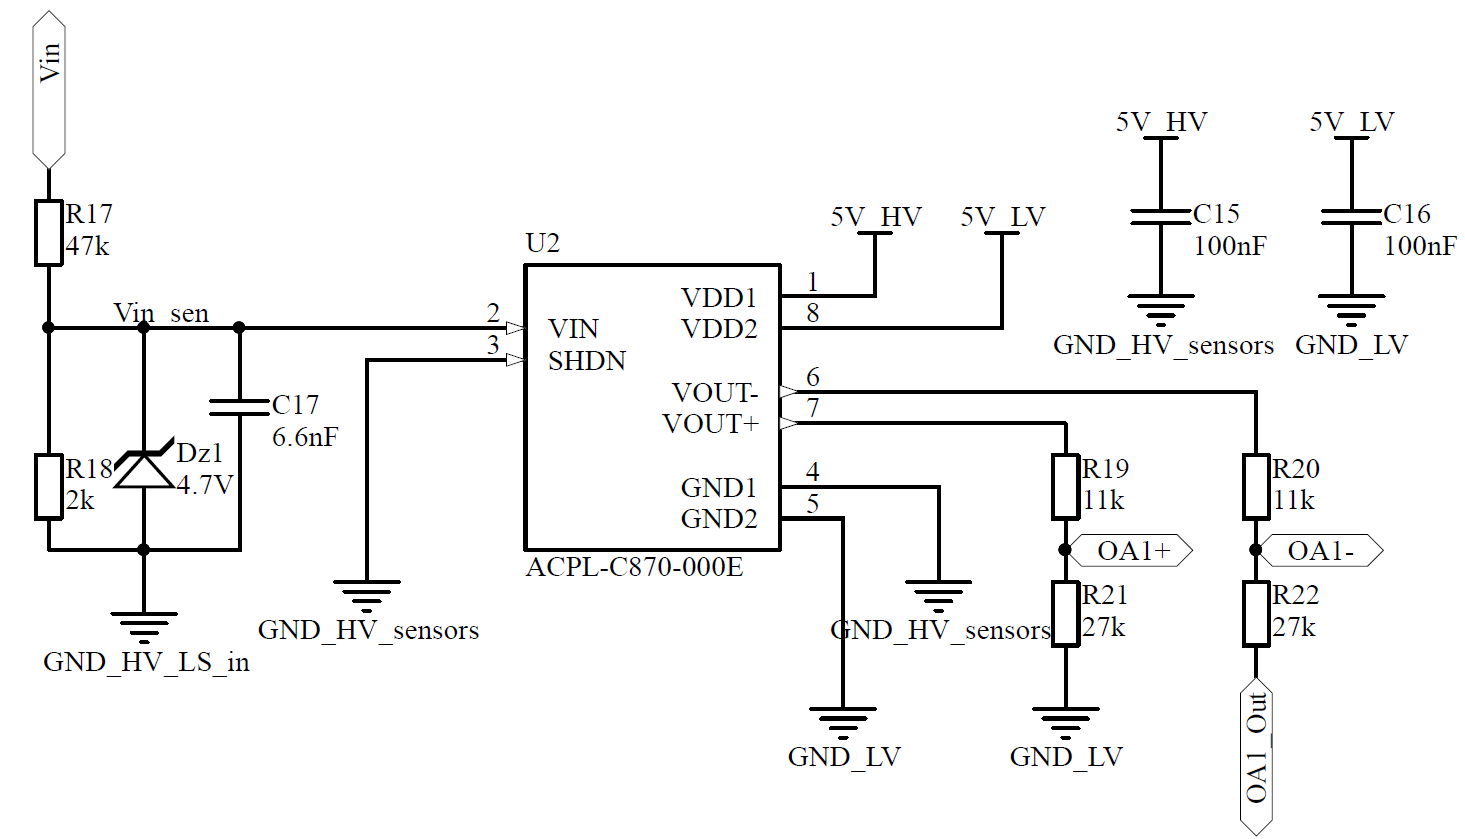
\includegraphics[width=0.7\linewidth]{../Pictures/P1/Sensors/input_voltage_sensor.PNG}
		\caption{Input voltage sensor}
		\label{fig:input_voltage_sensor_circuit}
	\end{center}
\end{figure}

\subsection{Output voltage sensor}
The voltage sensor at the output is design by the same procedure as the input sensor. The voltage divider will designed such that the values of the amplifier can be reused.

\subsubsection{Voltage divider}
The maximum output voltage of the DC/DC converter will be $90V$, when only 4 PV-modules are used. To insert a safety margin if one converter fails, the maximum sensed voltage will be designed at $120V$.

The resistors will be sized by reusing equation \ref{voltage_divider_R17_in} and \ref{voltage_divider_R18_in}.
\begin{equation}
	R_{26} = \frac{V_{in,max}-V_{out}}{I} = \frac{120V-2V}{1mA} = 118k\Omega	
\end{equation}

\begin{equation} 
	V_{out} = V_{in,max} \cdot \frac{R_{27}}{R_{26}+R_{27}} \Rightarrow 2V = 120V \cdot \frac{R_{27}}{118k\Omega+R_{27}}
\end{equation}
\begin{center}
	$R_{27} = 2.03k\Omega$
\end{center}

To achieve these resistor values $R_{26} = 120k\Omega$ and $R_{27} = 2k\Omega$ have been chosen. 

\subsubsection{Filtering}
The filter will be design with the same corner frequency at $500Hz$, as for the input sensor.

The resistor of the filter will be $R_{26}$ in the voltage divider. The capacitor will be calculated as followed in equation \ref{voltage_sensor_out_filter_cap}:
\begin{equation} \label{voltage_sensor_out_filter_cap}
	C_{22} = \frac{1}{2\pi \cdot f_c \cdot R_{26}} = \frac{1}{2 \pi \cdot 500Hz \cdot 120k\Omega} = 2.6nF
\end{equation}

To achieve the capacitance $C_{22} = 3.3nF$ has been chosen. 

\subsubsection{The circuit}
The circuit regarding the input voltage measurement is shown at figure \ref{fig:output_voltage_sensor_circuit}. $V_{out}$ is the measured voltage from the converter output. The points $OA2_+$ and $OA2_-$ are connected to the non-inverting and inverting input of the amplifier respectively. $OA2_{out}$ is connected to the output of the amplifier. $C_{20}$ and $C_{21}$ are decoupling capacitors for the two supply voltages. 

\begin{figure}[H]
	\begin{center}
		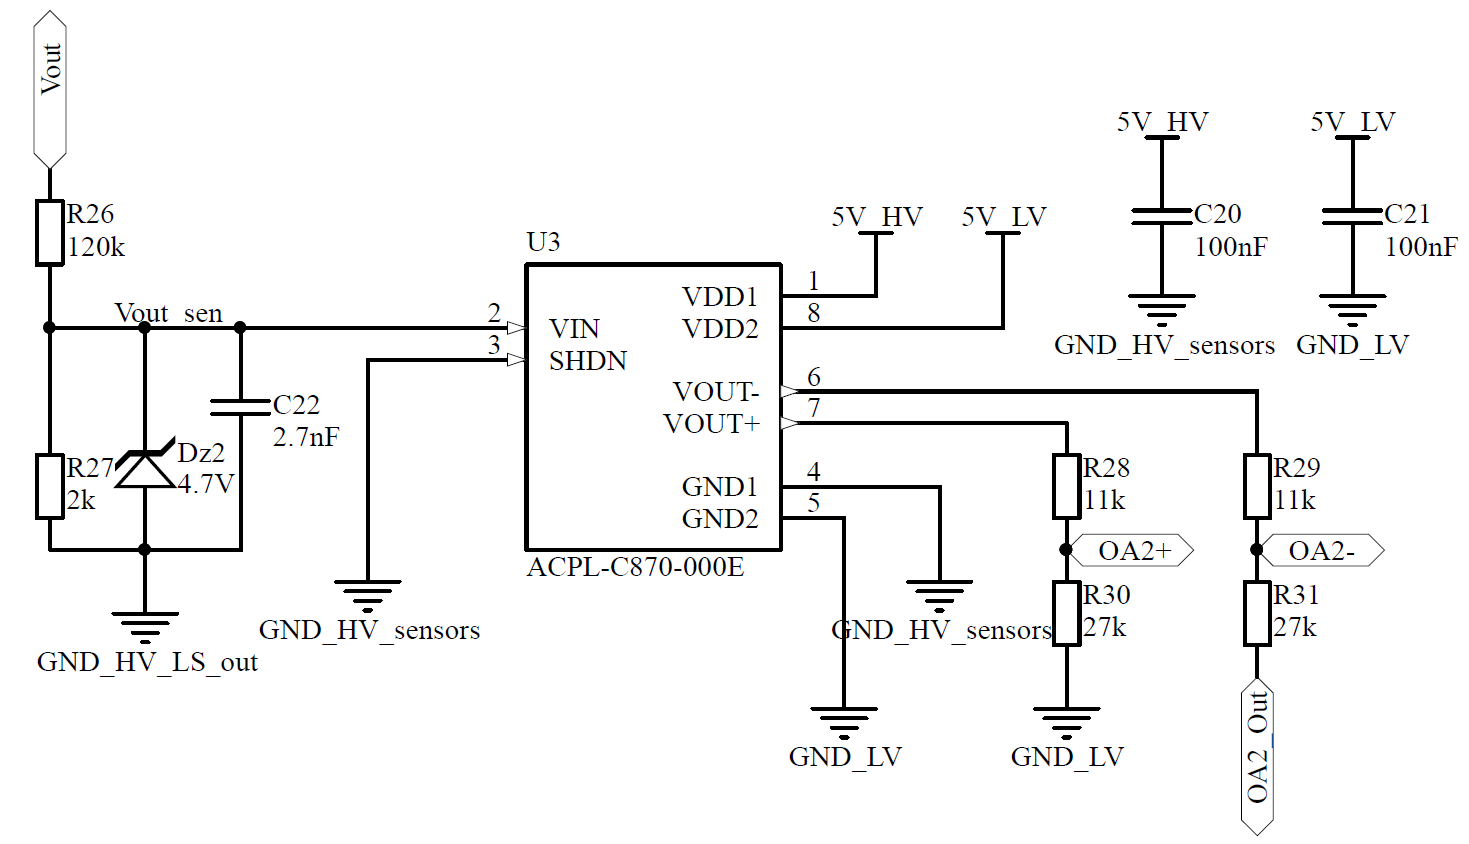
\includegraphics[width=0.7\linewidth]{../Pictures/P1/Sensors/output_voltage_sensor.PNG}
		\caption{Output voltage sensor}
		\label{fig:output_voltage_sensor_circuit}
	\end{center}
\end{figure}

%%% Current sensors %%%
\subsection{Current sensor} \label{current_sensor}

The current along with the voltage of the PV allows the system to perform power calculation, which is needed for the MPPT algorithm. The current will be measured in parallel with the inductor with a hall effect sensor. Placing it in series with the PV module would be the easiest approach for MPPT, but placing it in parallel with the inductor allows implementing a current controller for possible future use.

\begin{figure}[htbp]
	\begin{center}
		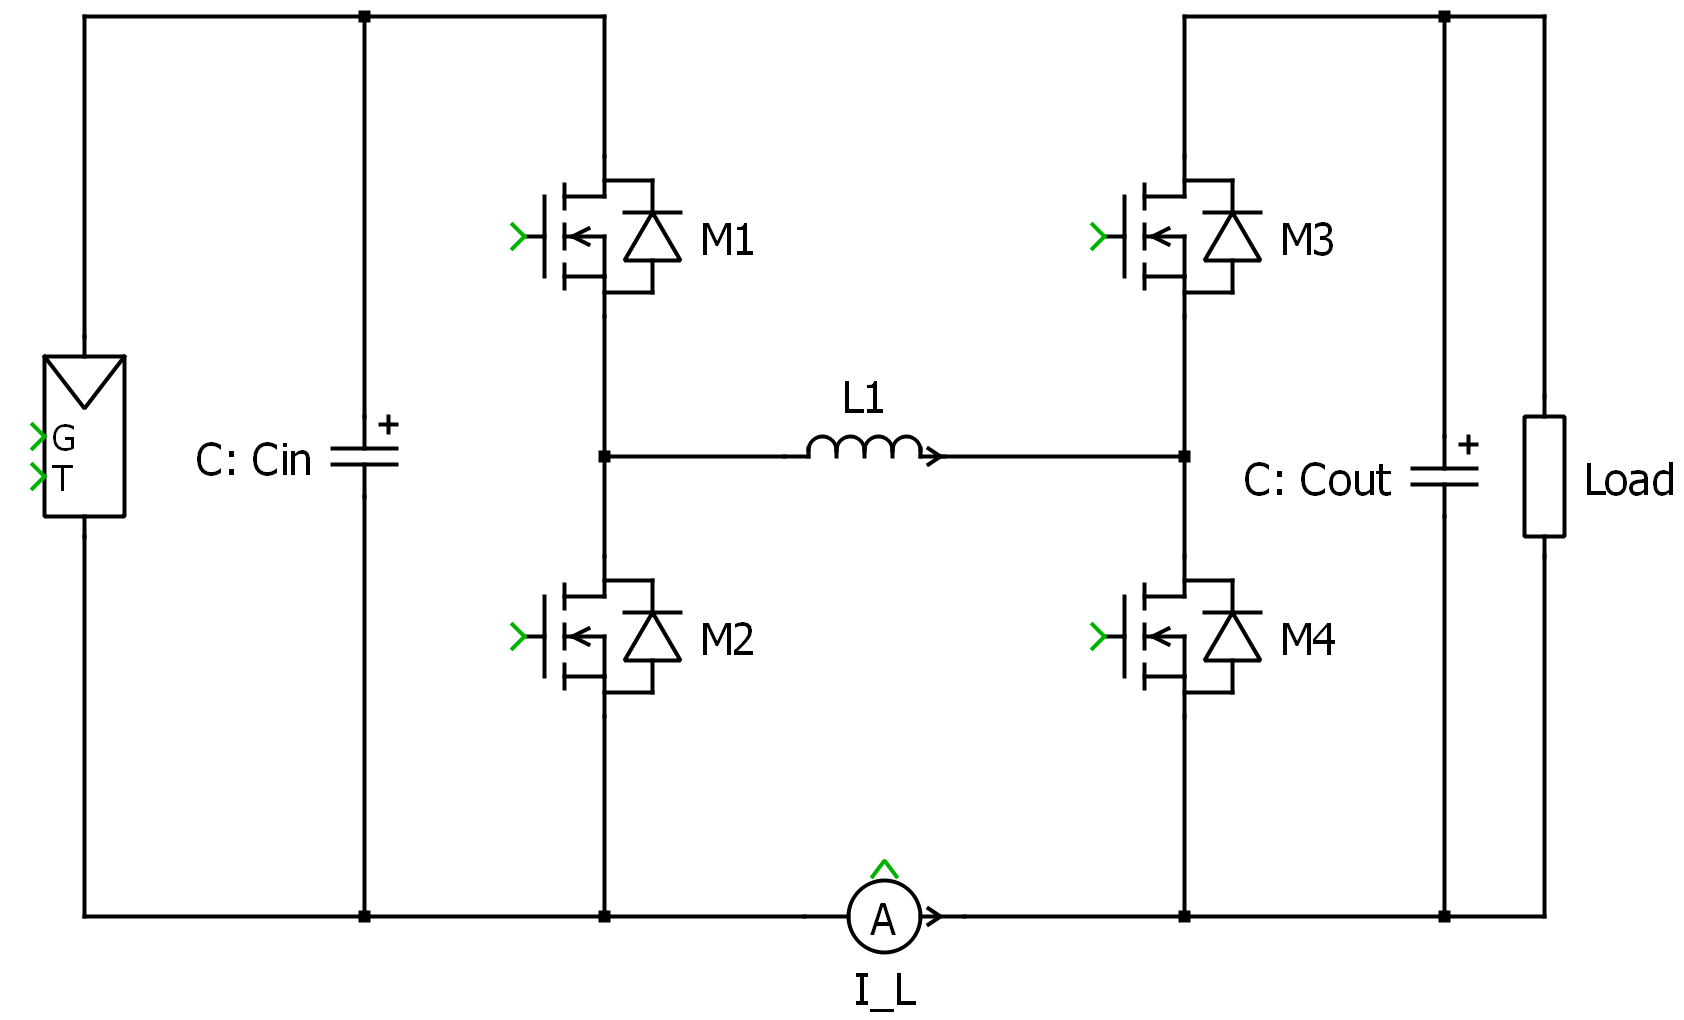
\includegraphics[width=0.4\textwidth]{../Pictures/current_sensor_placement.png}
		\caption{Current sensor placement.}
		\label{current_sensor_placement}
	\end{center}	
\end{figure}

The sensor is a ACS723-20AB which is a Hall effect sensor. Its features might be found in table \ref{current_sensor_features}.

\begin{table}[htbp]
	\centering
	\begin{tabular}{|p{6cm}|>{\centering}p{8cm}|}
		\hline
		\rowcolor{lightgray}\multicolumn{2}{|l|}{ \textbf{Maximum ratings}} \\ \hline
		Supply voltage & 4.5-5.5 [V]  \tabularnewline \hline
		Gain & 100 [mV/A]  \tabularnewline \hline
		Input range & $\pm$20 [A]  \tabularnewline \hline
		\rowcolor{lightgray}\multicolumn{2}{|l|}{ \textbf{Other values of interest}} \\ \hline
		Bandwidth & 20 or 80 [kHz]  \tabularnewline \hline
		Package & SOIC8  \tabularnewline \hline
		
	\end{tabular}
	\caption{Current sensor figures of merit. \cite{current_sensor}}
	\label{current_sensor_features}
\end{table}

The output of the sensor is a voltage proportional to the current following the next equation:
 \todo[inline,color=green]{maybe the gain is 0.125, to be confirmed by test.}
\begin{equation} 
V_{current} = \frac{1}{10} \, i + 2.5
\end{equation}

In order to ease the task of the control, the signals are filtered by hardware. The current will be used by the MPPT, which frequency is $100 Hz$ \todo{check final implementation}. The sensor output is filtered by a LPF which cut-off frequency is $500 Hz$. The cut-off frequency has been calculated by a hundredth of the switching frequency, which is $50 kHz$. Also the current might be used in the current controller, this signal will be filtered at $80 KHz$ in order to remove high frequency noise, this cut-off frequency was selected as it is the sensor's bandwidth. The filters are first order low-pass filters implemented with a resistor in series with a capacitor.\todo{has the current control been implemented? was enough this filtering?}

In order to calculate the current from the PV module, the converter working mode will have to be taken into account. Assuming continuous conduction mode, the average PV current is:


\begin{equation} 
	Buck \; mode \rightarrow \overline{I_{in}} = i_{measured} \cdot \delta
\end{equation}
\begin{equation} 
Boost \; mode \rightarrow \overline{I_{in}} = i_{measured} \cdot
\end{equation}
\begin{equation} 
Buck-Boost \; mode \rightarrow \overline{I_{in}} = i_{measured} \cdot \delta
\end{equation}

The IC has been placed far from the inductor in order to avoid undesired magnetic flux.

 


\section{Power Supplies}\label{power_supplies}
In the first iteration of the converter, the drivers and the sensors will be supplied by an external $12V$ voltage source. This source will be used directly to supply the two lower leg MOSFET drivers. To support the higher leg drivers, two isolating $12V$ supplies will be used, with the external $12V$ as input. These will be two TRACO supplies \textit{TMA1212S} \cite{traco_tma1212}. The chosen voltage sensors need a $5V$ power supply at both input and output of the sensor. These should be isolated from each other. The input side will be supplied by a $5V$ voltage regulator, \textit{LD1117} \cite{LD1117}, and the output side will be supplied by the RT-box \todo{consider changing if we are finally not able to supply from rt box. AT}. The current sensor will also be supplied with $5V$ by the RT-box. A LED will be added to every voltage source, to indicate if they are working.


\section{PCB design}
\subsection{PCB structure} \label{PCB_Schematic}
In order to proceed with the creation of the PCB, a schematic circuit has been designed. This compiles all the previously mentioned components as well as other components required for current limiting, decoupling, external connections, or safety components for protection. Both the PCB layout and schematics are found in appendix \ref{ch:AppPCB}.

The schematic has been divided into four main sections, these are \textit{main topology}, \textit{power supplies}, \textit{drivers} and \textit{signal processing}.

The main topology includes the power circuit, this is the MOSFETs, the inductor, the input and output capacitors and the input and output connectors. It also includes discharging resistors for the capacitors which have been sized for one minute discharge time. The gate of the MOSFETs is also connected to the source through a resistor designed for 3ms discharge time. These safety resistors are implemented in order to ensure that the circuit is fully discharged when disconnected. A series Schottky diode is included at the input to protect the components in case of reverse connection. However, this diode can be short-circuited at any moment.

The power supplies include the 12V external input connector and two isolated 12V supplies. These two are necessary to power the gates of the high side transistors and drivers. Lastly, a 5V linear regulator supply has also been connected to feed the sensors. This 5V signal is referred to the power ground, thus the input 5V signal could not be used since it does not share the same ground.

The drivers section is composed of the isolating optocouplers and the MOSFET gate drivers. The PWM signals to the optocouplers come directly from the RT Box, meaning that a connector is also included here. Decoupling capacitors are added in the vicinity of the ICs in order to assure that the current peaks needed by these are granted.

The signal processing section is composed by the IC sensors and the operational amplifier. As stated previously, there are 2 isolated voltage sensors and a hall effect sensor for current measuring. Also, voltage dividers are located in this section. These include protection zener diodes limiting 4.7V output voltage and filtering capacitors, amplification resistors are added. The current sensor also includes a selection pin header which will allow different filtering frequencies options. The operational amplifier is also included.

Finally, test points have been added to the signals that might be measured.


\input{docs/hardwareImplementation/PCB_layout/PCB_layout.tex}